% CVPR 2027 submission -- built on the official author kit (github.com/cvpr-org/author-kit)
\documentclass[10pt,twocolumn,letterpaper]{article}

%%%%%%%%% PAPER TYPE
\usepackage[review]{cvpr}      % REVIEW version (anonymous, line numbers)
% \usepackage{cvpr}            % camera-ready

%% This file contains a number of tweaks that are typically applied to the main document.
%% They are not enabled by default, but can be enabled by uncommenting the relevant lines.


%%
%% Official support for 2-column teaser figure
%%
\usepackage{cuted} %< for strip environment

%%
%% For auto-referencing of figures (see fig/teaser.tex and \label{} therein) 
%%
\usepackage{currfile} %< for \currfilebase macro

%%
%% caption and (global) spacing overrides
%%
\usepackage{caption} %< for "\captionof" commands (teaser)
% \setlength{\abovecaptionskip}{.5em} % space above caption
% \setlength{\belowcaptionskip}{1em} % space below caption

%%
%% Inline annotations; for predefined colors, refer to "dvipsnames" in the xcolor package:
%% https://tinyurl.com/overleaf-colors
%%
\newcommand{\red}[1]{{\color{red}#1}}
\newcommand{\todo}[1]{{\color{red}#1}}
\newcommand{\TODO}[1]{\textbf{\color{red}[TODO: #1]}}
%%
%% Disable for camera ready / submission by uncommenting these lines:
%%
% \renewcommand{\TODO}[1]{}
% \renewcommand{\todo}[1]{#1}

%%
%% Work harder in optimizing text layout. Typically shrinks text by 1/6 of page, enable
%% it at the very end of the writing process, when you are just above the page limit.
%%
% \usepackage{microtype}

%%
%% Fine-tune paragraph spacing.
%%
% \renewcommand{\paragraph}[1]{\vspace{.5em}\noindent\textbf{#1.}}

%%
%% Globally adjusts space between figure and caption.
%%
% \setlength{\abovecaptionskip}{.5em}

%%
%% Allows "the use of \paper to refer to the project name"
%% with automatic management of space at the end of the word.
%%
% \usepackage{xspace}
% \newcommand{\paper}{ProjectName\xspace}

%%
%% Commonly used math definitions.
%%
% \DeclareMathOperator*{\argmin}{arg\,min}
% \DeclareMathOperator*{\argmax}{arg\,max}

%%
%% Tighten underline.
%%
% \usepackage{soul}
% \setuldepth{foobar}

%%
%% Reconfigure paragraph (tweaks spacing)
%%

\usepackage{multirow}
\usepackage{makecell}
\usepackage{pifont}
\usepackage{amsthm}
\usepackage{algorithm}
\usepackage{algpseudocode}

\definecolor{cvprblue}{rgb}{0.21,0.49,0.74}
\usepackage[pagebackref,breaklinks,colorlinks,allcolors=cvprblue]{hyperref}

\def\confName{CVPR}
\def\confYear{2027}

% ---- macros -------------------------------------------------------------
\newtheorem{theorem}{Theorem}
\newtheorem{definition}{Definition}
\newcommand{\A}{\mathcal{A}}
\newcommand{\B}{\mathcal{B}}
\newcommand{\C}{\mathcal{C}}
\newcommand{\Lam}{\Lambda}
\newcommand{\ours}{CSI\xspace}               % Certified Self-Improvement
\newcommand{\cmark}{\ding{51}}
\newcommand{\xmark}{\ding{55}}
\newcommand{\CHECK}[1]{\textcolor{red}{[CHECK: #1]}}  % to be verified before submission
% expandable input for generated table bodies (plain \input breaks \multicolumn and \bottomrule)
\makeatletter\newcommand{\tabinput}[1]{\@@input #1 }\makeatother
\newcommand{\para}[1]{\vspace{2pt}\noindent\textbf{#1}\hspace{0.4em}}

% Set to \withsupplfalse to build the main paper alone.
\newif\ifwithsuppl
\withsuppltrue

%%%%%%%%% TITLE
\title{First, Do No Harm: Certified Self-Improvement for\\Medical Image Segmentation Under Domain Shift}

\author{Anonymous CVPR submission}

\begin{document}
\maketitle

\begin{abstract}
Segmentation models deployed on a new domain can be improved with a few labelled cases, but an update that helps on average can still silently harm individual patients.
We make self-improvement \emph{certifiable}: an update---to a refinement agent or to the segmentation model itself---is deployed only if a Learn-then-Test procedure bounds the fraction of patients it harms (a lost lesion or reduced Dice, relative to the deployed system) below a user-chosen tolerance $\delta$ with probability $1-\alpha$; otherwise the system rolls back.
We study an FDG PET/CT tumour-segmentation system transferred to an unseen tracer (PSMA, 377 patients), with disjoint adaptation, certification and locked test sets under a pre-registered protocol.
Zero-shot, the system is safe but poor (Dice 0.11).
Certified updates to the refinement agent help only modestly ($+0.009$ Dice, 0 of 125 test patients harmed).
Certified fine-tuning of the segmenter on 126 patients raises Dice from 0.11 to 0.55 and cuts false-positive volume by 98\% on the locked test; certified at $\delta=10\%$, it harms 2.4\% of test patients (95\% upper bound 6.1\%), while at our pre-registered $\delta=5\%$ the certificate refused the switch.
On the same patients, naive self-improvement harms 11 patients and loses 20 lesion detections, and pseudo-label self-training harms 4 without gain.
Across 1,000 resampled splits and three backbones, naive selection breaks a 5\% harm promise in at least 98\% of splits and certified selection in at most 0.7\%.
The tolerance $\delta$ thus becomes a dial that trades benefit for risk, with a guarantee at every setting.
\end{abstract}

\section{Introduction}
\label{sec:intro}

A segmentation model that leaves the site where it was trained meets a new scanner, a new protocol or, in nuclear medicine, a new radiotracer.
Its accuracy drops, and the receiving site usually holds a small labelled set with which it could adapt the model.
Adapting is the obvious move, and the computer-vision toolbox for it is rich: fine-tuning, test-time adaptation~\cite{sun2020ttt,wang2021tent,karani2021tta}, self-training~\cite{lee2013pseudo,xie2020noisy}, and, increasingly, agents that critique and repair their own outputs~\cite{madaan2023selfrefine,shinn2023reflexion}.
All of them are judged by an \emph{average}: mean Dice on a validation set.

In medicine the average is not the decision that matters.
An update that raises mean Dice can still delete a metastasis in one patient, and that patient is not consoled by the mean.
Clinicians state the requirement as ``first, do no harm''; regulators increasingly ask that a model's planned changes be specified, with their verification method, before they are made~\cite{fda2023pccp,feng2022monitoring}.
What is missing is a way to make an \emph{update decision} that carries a statement of the form: \emph{this update harms at most a fraction $\delta$ of future patients, and this statement is wrong with probability at most $\alpha$.}

\para{This paper.} We propose \textbf{Certified Self-Improvement} (\ours), a certify-before-deploy protocol for updating a deployed segmentation system (\cref{fig:overview}).
Candidate updates are built on an adaptation set $\A$.
Each candidate defines a null hypothesis ``its patient-level harm rate exceeds $\delta$'', which is tested on a disjoint certification set $\B$ with the Learn-then-Test (LTT) framework~\cite{angelopoulos2021ltt}; a candidate is deployed only if its hypothesis is rejected, and otherwise the system \emph{rolls back} to what is already deployed.
Harm is defined per patient and relative to the deployed system---a lesion that was detected and is no longer, or a Dice drop larger than $0.01$---so the guarantee speaks to exactly the event a clinician fears.
The protocol is agnostic to what the update is: we apply it both to a learned \emph{refinement agent} that edits the segmenter's output and to the \emph{segmenter's weights}.

\para{Testbed.} We transfer an FDG PET/CT tumour-segmentation system~\cite{gatidis2022autopet} to PSMA PET/CT, a different tracer with different physiological uptake, on 377 patients split into adaptation, certification and locked test sets (126/126/125).
Every analysis was pre-registered and every test arm was hash-locked before the test set was read, once.

\para{Findings.}
\textbf{(i)} Zero-shot, the system is safe but poor: Dice $0.11$ and over $700$\,mL of false-positive volume per scan.
\textbf{(ii)} Certified updates of the refinement agent are safe (0 of 125 test patients harmed) but small ($+0.009$ Dice): an agent that edits a poor segmentation cannot create a good one.
\textbf{(iii)} Certified fine-tuning of the segmenter lifts Dice from $0.11$ to $0.55$ and cuts false-positive volume by $98\%$ on the locked test.
At our pre-registered tolerance $\delta=5\%$ the certificate \emph{refused} this switch---4 of 126 certification patients were harmed---and at $\delta=10\%$ it accepted it; on the locked test 2.4\% of patients were harmed (95\% upper bound 6.1\%).
\textbf{(iv)} Without the certificate, the same machinery is dangerous: naive self-improvement harms 11 test patients and loses 20 lesion detections, pseudo-label self-training harms 4 with no gain, and over 1,000 resampled splits naive selection breaks a 5\% harm promise in $98.5$--$99.6\%$ of splits, against $0.2$--$0.5\%$ for \ours, on three segmentation backbones.

\para{Contributions.}
\begin{enumerate}[nosep,leftmargin=*]
\item A certify-before-deploy formulation of self-improvement for segmentation, with a \emph{patient-level, relative} harm risk and a finite-sample guarantee (\cref{sec:method}).
\item A pre-registered, locked study of self-improvement under a real clinical domain shift, at two levels---agent and segmenter---with naive, pseudo-label and uncalibrated baselines (\cref{sec:setup,sec:results}).
\item Evidence that the guarantee holds where naive selection fails, across three backbones, and where three further rules fail (\cref{sec:validity}); a patient-level analysis showing how averages hide harm (\cref{sec:patients}); and a \emph{risk--benefit dial} with its sample-size cost (\cref{sec:dial}).
\item An honest account of what certification cannot do: it bounds risk, it does not create benefit; the large gain comes from adapting the segmenter, and the guarantee costs samples (\cref{sec:discussion}).
\end{enumerate}

\begin{figure*}[t]
  \centering
  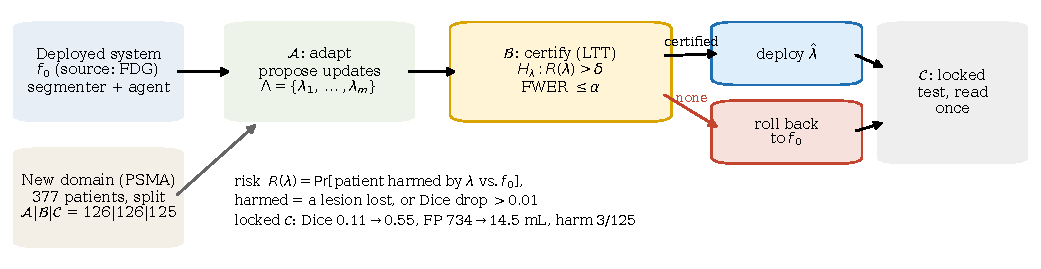
\includegraphics[width=\linewidth]{fig/fig_overview.pdf}
  \caption{\textbf{Certified Self-Improvement.}
  A deployed system $f_0$ meets a new domain.
  Candidate updates $\Lam$ (refinement-agent policies or segmenter weights) are built on the adaptation set $\A$ only.
  On the certification set $\B$, each $\lambda$ is a hypothesis $H_\lambda: R(\lambda)>\delta$, where $R$ is the probability that $\lambda$ harms a patient relative to $f_0$; Learn-then-Test rejects a subset with family-wise error at most $\alpha$.
  The most beneficial certified update is deployed; if none is certified the system rolls back to $f_0$.
  The locked test set $\C$ is read once.
  Numbers: segmenter-level update, PSMA PET/CT, locked $\C$ (\cref{tab:main}).}
  \label{fig:overview}
\end{figure*}

\section{Related Work}
\label{sec:related}

\para{Distribution-free risk control.}
Conformal prediction~\cite{vovk2005alrw,angelopoulos2021gentle} and its risk-control descendants~\cite{bates2021rcps,angelopoulos2024crc,angelopoulos2022image2image} calibrate a \emph{prediction} so that an expected loss is bounded.
Learn-then-Test (LTT)~\cite{angelopoulos2021ltt} recasts the choice of hyper-parameters as multiple hypothesis testing, which allows non-monotone risks and arbitrary families.
We use LTT for a different object: not the output of one model, but the \emph{decision to replace} a deployed model by another, with a risk defined per patient and relative to what is deployed.
We are not aware of a prior locked, pre-registered evaluation of certified model updates under a real clinical domain shift.

\para{Adaptation under domain shift.}
Unsupervised and test-time adaptation~\cite{ganin2016dann,sun2020ttt,wang2021tent} and their medical variants~\cite{karani2021tta} improve average accuracy without target labels; self-training~\cite{lee2013pseudo,xie2020noisy} uses the model's own predictions as labels.
Fine-tuning with a few target labels is the strongest practical option.
All of these optimise or select by an average, and none states how many patients an update may harm; we show (\cref{sec:main}) that average-driven selection harms patients that a certificate protects.
Continual learning~\cite{kirkpatrick2017ewc} protects the \emph{source} task; we protect \emph{individual target patients}.

\para{Uncertainty, quality control and refinement.}
Segmentation uncertainty~\cite{kendall2017uncertainties,lakshminarayanan2017ensembles,jungo2019reliability} and calibration~\cite{guo2017calibration,mehrtash2020calibration} underpin automatic quality control~\cite{kohlberger2012evaluating,robinson2019automated} and selective prediction~\cite{geifman2017selective}.
Interactive and automatic refinement~\cite{wang2019deepigeos} and self-refining agents~\cite{madaan2023selfrefine,shinn2023reflexion} edit an output after the fact.
Our refinement agent belongs to this line; our contribution is the rule that decides when such an agent, or the model beneath it, may change.

\para{Safe deployment and pre-registration.}
Proposals for monitoring and updating clinical AI~\cite{feng2022monitoring} and regulatory change-control plans~\cite{fda2023pccp} ask for pre-specified update protocols.
Pre-registration~\cite{nosek2018preregistration} guards against analytic flexibility; we pre-register every decision rule and lock every test arm by hash before the test set is read.

\section{Certified Self-Improvement}
\label{sec:method}

\subsection{Setting and patient-level harm}
\label{sec:harm}

A system $f_0$ is deployed on a new domain.
Patients $i$ are drawn i.i.d.\ from the new domain, and labelled patients are split once into an adaptation set $\A$, a certification set $\B$ ($|\B|=n$) and a locked test set $\C$.
From $\A$ alone we build a finite family $\Lam$ of candidate updates; candidate $\lambda$ produces the system $f_\lambda$.

\begin{definition}[Patient harm]
For patient $i$ with ground-truth lesions $G_i$, let $\mathrm{hit}_i(f)$ be the number of lesions in $G_i$ touched by the prediction of $f$, and $\mathrm{Dice}_i(f)$ its Dice score.
Update $\lambda$ \emph{harms} patient $i$, $H_i(\lambda)=1$, if
\begin{equation}
\mathrm{hit}_i(f_\lambda)<\mathrm{hit}_i(f_0)\;\;\lor\;\;\big(G_i\neq\emptyset\,\land\,\mathrm{Dice}_i(f_\lambda)<\mathrm{Dice}_i(f_0)-\varepsilon\big),
\label{eq:harm}
\end{equation}
with $\varepsilon=0.01$. The risk of $\lambda$ is $R(\lambda)=\Pr[H(\lambda)=1]$.
\end{definition}

Three choices are deliberate.
The unit is the \emph{patient}, the unit of clinical consequence, not the voxel or the lesion.
Harm is \emph{relative to $f_0$}: the question at deployment is whether replacing the current system hurts anyone, not whether the new one is perfect.
And harm is \emph{asymmetric}: a large Dice gain in one patient does not offset a lost lesion in another, so an update with excellent mean Dice can have a high risk.
The rollback $\lambda_0\!:=\!f_0$ has $R(\lambda_0)=0$ by definition.

\subsection{Certification by Learn-then-Test}
\label{sec:ltt}

For each $\lambda\in\Lam$ we test $H_\lambda: R(\lambda)>\delta$ on $\B$.
With $k_\lambda=\sum_{i\in\B}H_i(\lambda)$, the exact binomial p-value
\begin{equation}
p_\lambda=\Pr\big[\mathrm{Bin}(n,\delta)\le k_\lambda\big]
\label{eq:pval}
\end{equation}
is super-uniform under $H_\lambda$~\cite{angelopoulos2021ltt}.
Candidates are organised into $m$ \emph{chains}, each ordered from conservative to aggressive (\eg, an action gate lowered step by step); within a chain we use fixed-sequence testing, stopping at the first non-rejection, and each chain is tested at level $\alpha/m$~\cite{bretz2010multiple}.
Let $\hat\Lam\subseteq\Lam$ be the rejected (certified) set.
The deployed update is the certified candidate with the largest measured benefit on $\B$ (subject to a minimum support), or the rollback if $\hat\Lam=\emptyset$.

\begin{theorem}[Single-round guarantee]
If patients in $\B$ and future patients are exchangeable, and $\Lam$ is constructed without $\B$, then the deployed $\hat\lambda$ satisfies
$\Pr\big[R(\hat\lambda)>\delta\big]\le\alpha$.
\label{thm:ltt}
\end{theorem}
\noindent\emph{Proof sketch.} Every $p_\lambda$ is super-uniform under $H_\lambda$; fixed-sequence testing within chains and Bonferroni across them control the family-wise error at $\alpha$; $\hat\lambda$ is either certified or the zero-risk rollback.
Selection by benefit happens only \emph{among} certified candidates, so it cannot inflate the error (\cref{sec:supp_proof}). \hfill$\square$

\para{Power.} With $k=0$ harms, $H_\lambda$ is rejected only if $(1-\delta)^n\le\alpha/m$.
The smallest certifiable tolerance is therefore $\delta_{\min}=1-(\alpha/m)^{1/n}$: for $n=126$ and $m=8$ chains, $\delta_{\min}=0.040$.
The certificate is honest about sample size: a 1\% guarantee needs several hundred certification patients (\cref{fig:power}a).
Because $\delta$ is a free parameter, sweeping it gives a \emph{risk--benefit dial}: for each tolerance, the best certified update and its benefit.

\para{Why a test, and why per patient.}
Comparing mean Dice on $\B$ (``validate and pick the best'') asks whether an update is better \emph{on average}, so a lost lesion in one patient is outweighed by small gains in many; bounding an expected per-patient loss~\cite{angelopoulos2024crc} allows the same trade.
Our risk is the probability of an \emph{event} that no gain elsewhere offsets, and the rule bounds the probability that this risk exceeds $\delta$ (alternatives in \cref{sec:supp_faq}).
\Cref{alg:csi} summarises the procedure.

\begin{algorithm}[t]
\caption{Certified Self-Improvement (one round)}
\label{alg:csi}
\small
\begin{algorithmic}[1]
\Require deployed $f_0$; disjoint $\A$, $\B$ ($|\B|=n$); tolerance $\delta$; level $\alpha$; harm rule (Eq.~\ref{eq:harm})
\State Build candidates $\Lam$ on $\A$ only; order them into $m$ chains, conservative first
\For{each chain $c=1,\dots,m$}
  \For{$\lambda$ in chain $c$, in order}
    \State $k_\lambda\gets\sum_{i\in\B}H_i(\lambda)$ \Comment{harm relative to $f_0$}
    \State $p_\lambda\gets\Pr[\mathrm{Bin}(n,\delta)\le k_\lambda]$
    \If{$p_\lambda\le\alpha/m$} add $\lambda$ to $\hat\Lam$ \Else{} \textbf{break} \EndIf
  \EndFor
\EndFor
\State \Return $\arg\max_{\lambda\in\hat\Lam}\mathrm{benefit}_\B(\lambda)$ if $\hat\Lam\neq\emptyset$, else $f_0$ (rollback)
\end{algorithmic}
\end{algorithm}

\subsection{Two levels of self-improvement}
\label{sec:levels}

\para{Level 1: the refinement agent.}
On top of the segmenter runs an agent that diagnoses and repairs its output (details in \cref{sec:supp_agent}).
Each connected component of the prediction is described by 26 image and model features plus 21 context features (local tumour-to-background ratio, CT texture, anatomical neighbourhood, left--right symmetry, predicted-probability profile).
Gradient-boosted detectors estimate, per component, the probability of eight failure classes (\eg, physiological false positive, under-segmentation); a hand-built policy maps the predicted class to a repair action (removal, regrowth, threshold refinement), applied when the detector's confidence exceeds a gate.
This hand-built agent is the deployed $f_0$ in the new domain.
A candidate update \emph{adds} actions to it but never removes one (an anchored, one-sided trust region), using detectors refitted on $\A$ with isotonic calibration~\cite{guo2017calibration} on cross-fitted predictions, an out-of-distribution fence on the number of components per scan, and optional guards (agreement of old and new detectors; never act on a scan's only component).
The family is
$\Lam_{\text{agent}}=\{\text{detector}\}\times\{\text{guard}\}\times\{\text{gate}\}$, with 2 detectors, 4 guards and 11 gates ($0.99\to0.85$), \ie, $m=8$ chains and 88 candidates.
Per-patient harm on $\B$ is computed from the measured outcome of every action on every component.

\para{Level 2: the segmenter.}
The segmenter is fine-tuned on $\A$ (5 folds; each fold initialised from the corresponding source-domain model, all weights including the head; 100 epochs; nnU-Net defaults otherwise~\cite{isensee2021nnunet}).
The 5-fold ensemble gives the candidate FT, and FT followed by the hand-built agent gives FT+agent; $\Lam_{\text{seg}}=\{\text{FT},\text{FT+agent}\}$, each tested at $\alpha/2$ against the system deployed after Level 1.
Out-of-fold predictions on $\A$ let the Level-1 machinery be re-run on top of FT.

\para{Sequential deployment.}
Each round certifies against the system deployed by the previous round, so the chain of promises reads $f_0\to f_1\to f_2$.
Each round's guarantee holds at $\alpha$; a union bound gives a joint guarantee at $2\alpha$ for both rounds.

\section{Experimental Protocol}
\label{sec:setup}

\para{Source domain.} The source system was built on the AutoPET FDG PET/CT data~\cite{gatidis2022autopet} (1,014 studies; whole-body PET/CT with manually annotated lesions), with a patient-grouped split into 738 cross-validation, 76 validation and 200 test scans.
The segmenter is nnU-Net~\cite{isensee2021nnunet} (3D full resolution, plain convolutional U-Net) initialised from a masked-autoencoder PET/CT model~\cite{he2022mae,liu2026petctmae}, trained as a 5-fold ensemble (source test Dice $0.664$).
The refinement agent and its detectors were developed on source cross-validation data only (\cref{sec:supp_fdg}).

\para{Target domain.} PSMA-PET-CT-Lesions~\cite{psma2025tcia} from TCIA~\cite{clark2013tcia}: 597 studies of 377 patients with prostate cancer, two radionuclides ($^{18}$F, 213 patients; $^{68}$Ga, 164) and two scanner vendors.
We use one study per patient (the earliest), resampled to the source grid, so patients are independent.
PSMA differs sharply from FDG: intense physiological uptake in salivary glands, kidneys, bowel and bladder, and many small bone and nodal lesions.
The 377 patients are split once (seed fixed in advance, stratified by radionuclide $\times$ tumour status) into $\A/\B/\C$ $=126/126/125$; $\C$ holds 119 tumour-positive patients with 4,518 lesions.

\para{Pre-registration and locks.} For every phase, a plan fixing candidates, $\delta$, $\alpha$, endpoints and failure criteria was committed before any number it governs was computed.
Before $\C$ was read, a lock commit recorded the SHA-256 of every input table and the exact commands; each arm was then run once.
The certification tolerance was $\delta=0.05$, $\alpha=0.05$ for both levels; the dial values $\delta\in\{0.03,\dots,0.20\}$ were pre-registered as secondary.
All deviations are listed in \cref{sec:supp_deviations}.
The per-patient, subgroup and harm-definition analyses of \cref{sec:patients,sec:harmdef} were not pre-registered; they re-read the locked per-patient outputs, are descriptive, and change no decision.
One is material and we state it here: $\C$ was read for the Level-1 arms before the Level-2 plan was written. No Level-2 choice used $\C$---the fine-tuning recipe was fixed in the plan and certification used $\B$---but $\C$ is not virgin for Level 2.

\para{Baselines} (all on the same split, each locked and run once):
\textbf{Naive self-improvement} deploys the candidate with the largest mean benefit on $\B$, with no harm test---the standard ``validate and pick the best'' practice.
\textbf{Pseudo-label self-training}~\cite{lee2013pseudo} refits the detectors on $\A$ using the deployed detector's own predictions as labels (no target labels).
\textbf{Uncalibrated \ours} runs the full certificate on raw detector probabilities, isolating the role of calibration.

\para{Metrics.} Dice is averaged over tumour-positive patients; false-positive (FP) and false-negative volumes over all patients; lesion detection counts ground-truth lesions touched by the prediction; HD95 over tumour-positive patients.
Paired differences use a patient bootstrap (2,000 resamples, 95\% percentile intervals); harm rates use exact binomial tests and Clopper--Pearson upper bounds (UB)~\cite{clopper1934use}.

\para{Implementation.} The primary and the fine-tuned segmenters are 5-fold ensembles with flip test-time augmentation, run on a single 32\,GB GPU; Level-2 fine-tuning takes about 9\,GPU-hours in total.
Detectors are gradient-boosted trees (depth 3, 200 iterations) with isotonic calibration fitted on cross-fitted predictions; certification, the agent and all statistics run on CPU (the agent takes 7--10\,s per scan).
Full recipes are in \cref{sec:supp_agent,sec:supp_level2,sec:supp_repro}.

\section{Results}
\label{sec:results}

\begin{table*}[t]
\centering
\caption{\textbf{Locked test set $\C$} (PSMA PET/CT, 125 patients; 119 tumour-positive, 4,518 lesions). Each arm was hash-locked before $\C$ was read and run once.
$\Delta$Dice: paired difference to the zero-shot system with 95\% bootstrap interval.
Harmed: patients harmed relative to the system deployed at that level (Eq.~\ref{eq:harm}), with the exact one-sided 95\% upper bound (UB) on the harm rate.
Level 1 is certified at $\delta=0.05$; Level 2 at $\delta=0.10$ (at the pre-registered $\delta=0.05$ the switch was refused and the system rolled back to the Level-1 output; \cref{sec:main}).
Best certified result in \textbf{bold}.}
\label{tab:main}
\setlength{\tabcolsep}{5pt}
\small
\begin{tabular}{@{}lccccccc@{}}
\toprule
arm & cert. & Dice $\uparrow$ & \makecell{$\Delta$Dice vs.\ zero-shot\\{\scriptsize[95\% CI]}} & \makecell{FP\\mL $\downarrow$} & \makecell{lesions\\det.\ $\uparrow$} & \makecell{HD95\\mm $\downarrow$} & \makecell{harmed / 125\\(UB) $\downarrow$} \\
\midrule
zero-shot segmenter & -- & 0.107 & -- & 733.9 & 2092 & 198.0 & -- \\
\midrule
\multicolumn{8}{@{}l}{\emph{Level 1: refinement-agent updates} (reference: deployed agent $f_0$)} \\
deployed agent $f_0$ & -- & 0.109 & $+0.002$ {\scriptsize[$+0.000$, $+0.004$]} & 719.2 & 2094 & 198.0 & -- \\
naive self-improvement & \xmark & 0.236 & $+0.129$ {\scriptsize[$+0.094$, $+0.170$]} & 196.1 & 2074 & 147.1 & 11 (14.1\%) \\
pseudo-label self-training & \xmark & 0.108 & $+0.001$ {\scriptsize[$-0.001$, $+0.003$]} & 739.9 & 2094 & 198.2 & \phantom{0}4 (7.2\%) \\
\ours, uncalibrated & \cmark & 0.129 & $+0.022$ {\scriptsize[$+0.010$, $+0.037$]} & 505.1 & 2093 & 194.3 & \phantom{0}1 (3.7\%) \\
\ours (deployed as $f_1$) & \cmark & 0.116 & $+0.009$ {\scriptsize[$+0.004$, $+0.015$]} & 592.4 & 2094 & 194.0 & \phantom{0}0 (2.4\%) \\
\midrule
\multicolumn{8}{@{}l}{\emph{Level 2: segmenter update} (reference: Level-1 system $f_1$)} \\
\ours: fine-tuned segmenter & \cmark & \textbf{0.547} & $\mathbf{+0.440}$ {\scriptsize[$+0.396$, $+0.484$]} & \textbf{14.5} & \textbf{3547} & 90.9 & \phantom{0}3 (6.1\%) \\
\ours: fine-tuned + agent & \cmark & \textbf{0.549} & $+0.442$ {\scriptsize[$+0.398$, $+0.486$]} & \textbf{14.3} & 3530 & \textbf{75.9} & \phantom{0}3 (6.1\%) \\
\bottomrule
\end{tabular}
\end{table*}

\subsection{Zero-shot transfer is safe but poor}
\label{sec:zeroshot}
Transferred unchanged, the source segmenter reaches Dice 0.10 on PSMA and predicts 732\,mL of false-positive volume per scan, most of it physiological uptake in salivary glands, kidneys and bladder (\cref{fig:qual}).
The source-domain agent, also frozen, harms no one---0 of 377 patients (95\% UB 0.8\%)---but changes Dice by only $+0.001$.
A refinement agent built on FDG cannot repair a segmenter that was never shown PSMA; the system must change.

\subsection{Main result}
\label{sec:main}
\Cref{tab:main} reports every arm on the locked test set.

\para{Level 1: certified agent updates are safe and small.}
On $\B$, LTT certified 22 of the 88 agent updates (all with zero harmed patients on $\B$); the deployed one (calibrated detector, gate 0.97, both guards) adds 63 actions on $\C$.
On the locked test it harms none of the 125 patients ($p=0.0016$ against $R>0.05$; UB 2.4\%), loses no lesion, cuts FP volume by 127\,mL per scan ($[-186,-74]$; $-18\%$) and improves Dice over the deployed agent by $+0.0068$ ($[+0.0022,+0.0126]$, $p<0.001$).
Both pre-registered primary endpoints are met.
The gain is real and small: removing false positives from a segmentation that misses half the lesions cannot produce a good segmentation.

\para{Without the certificate, self-improvement harms patients.}
Naive self-improvement---the update with the best mean benefit on $\B$---obtains much higher Dice (0.236) by removing aggressively, but harms 11 test patients (8.8\%) and loses 20 lesion detections.
The harm was visible on $\B$ (13 patients, 22 lesions) to anyone who looked per patient; mean benefit does not look.
Pseudo-label self-training harms 4 patients, \emph{increases} FP volume and gains nothing: without target labels the detectors learn their own source-domain mistakes.
The uncalibrated certified variant gains more than calibrated \ours (+0.022) and harms 1 patient, within its guarantee: the certificate, not calibration, is what bounds the risk, and we do not credit calibration with the gain.

\para{Level 2: certifying the segmenter.}
Fine-tuning on the 126 adaptation patients changes the picture (\cref{tab:main}, bottom; \cref{fig:qual}).
On the locked test, Dice rises from 0.107 to 0.547 ($+0.440$, $[+0.396,+0.484]$; 110 of 119 tumour-positive patients improve by more than 0.01, one worsens), FP volume falls from 734 to 14.5\,mL per scan ($-98\%$), lesion detection rises from 2,092 to 3,547 of 4,518 lesions, and HD95 halves.
The agent on top of the fine-tuned segmenter adds almost nothing ($+0.002$ Dice), and no learned agent update could be certified on top of it.

\emph{The certificate's decision.}
On $\B$, the fine-tuned segmenter harmed 4 of 126 patients relative to the Level-1 system ($p=0.24$ against $R>0.05$ at $\alpha/2$; \cref{fig:l2B}), while improving 107 of the 120 tumour-positive ones by more than 0.01 Dice.
At the pre-registered $\delta=0.05$ the switch was therefore \textbf{refused} and the system rolled back---by the rule we fixed in advance, the primary Level-2 endpoint failed.
At $\delta=0.10$ the switch is certified ($p=0.004$) and on $\C$ it harms 3 of 125 patients (2.4\%; UB 6.1\%, below 10\%).
We read this as the certificate working rather than failing: with 126 patients, 4 harms are not enough evidence for a 5\% promise, and a site that wants the 0.44 Dice gain must either accept a 10\% tolerance or certify on more patients.
Two of the three harmed test patients had one or two small lesions that the Level-1 system ``detected'' only through spurious overlap (Dice 0.011) and the fine-tuned model missed; the third doubled its Dice (0.27$\to$0.60) but lost 4 of 106 detected lesions.
The harm definition is strict by design, and we keep it.

\begin{figure*}[t]
  \centering
  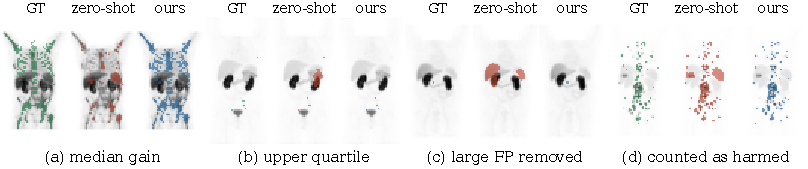
\includegraphics[width=\linewidth]{fig/fig_qual.pdf}
  \caption{\textbf{Locked test patients}, coronal PET maximum-intensity projections with ground truth (green), the zero-shot FDG segmenter (red) and the certified fine-tuned segmenter (blue).
  (a, b) Patients at the median and upper quartile of the Dice gain. (c) Physiological kidney uptake segmented as tumour zero-shot (862\,mL) and removed after certified fine-tuning. (d) One of the three patients counted as \emph{harmed}: Dice rises from 0.27 to 0.60 and FP volume falls from 314 to 3\,mL, yet 4 of 106 detected lesions are lost.}
  \label{fig:qual}
\end{figure*}

\begin{figure}[t]
  \centering
  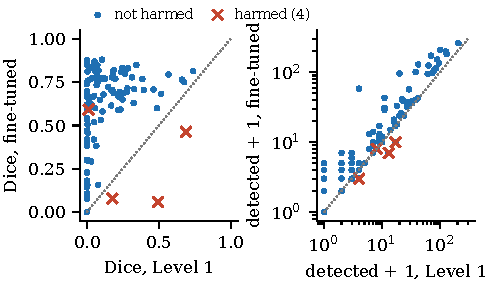
\includegraphics[width=\linewidth]{fig/fig_l2_B.pdf}
  \caption{\textbf{The Level-2 decision, on the certification set $\B$} (126 patients; the test set plays no part). Each point is a patient, Level-1 system ($x$) against fine-tuned segmenter ($y$). Left: Dice. Right: detected lesions (log scale, $+1$). Four patients are harmed (red): three lose detections, one loses Dice. Four of 126 cannot support a 5\% promise, so the switch is refused at $\delta=0.05$ and certified at $\delta=0.10$.}
  \label{fig:l2B}
\end{figure}

\subsection{Patient by patient}
\label{sec:patients}
Means hide what the certificate is about, so we look at every test patient (\cref{fig:patients}; descriptive, \cref{sec:setup}).

\para{Harm is invisible to the average.}
Naive self-improvement improves 49 patients by more than 0.01 Dice, worsens one, and still harms 11 (\cref{fig:patients}a).
All 11 lose lesions, and in 7 of them Dice \emph{rises} (by up to $+0.44$): removing a false-positive region that overlapped a lesion raises Dice and deletes the detection, and a mean-Dice criterion rewards exactly that.
Certified \ours improves 10 patients and harms none.

\para{Level 2 helps almost everyone.}
After certified fine-tuning (\cref{fig:patients}b,c) the median patient's Dice is 0.63, and 77 of 119 tumour-positive patients exceed 0.5 (5 before).
Lesion-level sensitivity rises from 46\% to 79\%: 1,460 detections are gained and 7 lost, all in the three harmed patients.
Two patients keep more than 100\,mL of false-positive volume (104 before).
\para{No subgroup is left behind.}
By radionuclide, scanner vendor and tumour burden (\cref{tab:subgroups}; full table in \cref{tab:supp_sub}), the gain ranges from $+0.36$ to $+0.49$ Dice with every interval above zero, and no subgroup has more than 2 harmed patients.
The weakest starting points gain most: vendor 1 (Level-1 Dice 0.06) and patients with one or two lesions (0.01) both reach about 0.5.
Harm, however, sits where the margin is thinnest: two of the three harmed patients have one or two lesions, where a single lost lesion is the patient's whole disease.
The residual false-positive volume is concentrated in the highest-burden patients (39\,mL per scan, against 2--4\,mL for patients with fewer lesions).

\begin{table}[t]
\centering
\caption{\textbf{Level 2 by subgroup} (locked $\C$, post hoc). Dice over tumour-positive patients, Level-1 system $\to$ certified fine-tuned segmenter; $\Delta$ with 95\% bootstrap interval; harmed relative to the Level-1 system. Vendors numbered by cohort size; burden in tertiles of lesion count.}
\label{tab:subgroups}
\footnotesize
\setlength{\tabcolsep}{3pt}
\begin{tabular}{@{}lcccc@{}}
\toprule
subgroup & $n$ & Dice & $\Delta$Dice {\scriptsize[95\% CI]} & harmed \\
\midrule
all & 125 & 0.116$\to$0.547 & $+0.431$ {\scriptsize[$+0.388$, $+0.475$]} & 3 \\
\midrule
$^{18}$F & 71 & 0.125$\to$0.551 & $+0.426$ {\scriptsize[$+0.376$, $+0.479$]} & 1 \\
$^{68}$Ga & 54 & 0.103$\to$0.541 & $+0.438$ {\scriptsize[$+0.361$, $+0.507$]} & 2 \\
vendor 1 & 55 & 0.061$\to$0.521 & $+0.460$ {\scriptsize[$+0.380$, $+0.532$]} & 2 \\
vendor 2 & 70 & 0.160$\to$0.568 & $+0.408$ {\scriptsize[$+0.357$, $+0.455$]} & 1 \\
1--2 lesions & 41 & 0.011$\to$0.453 & $+0.442$ {\scriptsize[$+0.348$, $+0.537$]} & 2 \\
3--24 lesions & 38 & 0.049$\to$0.543 & $+0.493$ {\scriptsize[$+0.434$, $+0.548$]} & 0 \\
$\ge$25 lesions & 40 & 0.286$\to$0.647 & $+0.361$ {\scriptsize[$+0.305$, $+0.416$]} & 1 \\
\bottomrule
\end{tabular}
\end{table}

\subsection{Does the conclusion depend on the harm definition?}
\label{sec:harmdef}
The harm event (\cref{eq:harm}) is a choice, fixed before any PSMA number was computed.
To see whether our conclusions rest on it, we recount harm for every locked arm under six alternatives (\cref{tab:harmdef}; post hoc, descriptive).
Two things hold under all of them.
Certified \ours harms no test patient.
And the Level-2 decision is unchanged: the fine-tuned segmenter harms 3 or 4 of the 126 certification patients, so it is refused at $\delta=0.05$ ($p\ge0.12>\alpha/2$) and certified at $\delta=0.10$ ($p\le0.004$).
Naive selection harms 11 patients whenever a single lost lesion counts, and still 5--7 when only larger losses do.

The instructive row is the Dice-only definition.
Under it naive selection harms a \emph{single} patient: a safety check based on segmentation overlap alone would see almost none of its harm, because it is lesion loss hidden inside a Dice gain (\cref{sec:patients}).
The opposite extreme, $\varepsilon=0$, counts numerical noise as harm: pseudo-labelling then ``harms'' 39 patients through Dice changes below 0.01.
One caveat: at Level 1 a different definition would also change \emph{which} updates certify on $\B$; the stored outputs of the locked arms cannot show that, so \cref{tab:harmdef} evaluates the decisions we made, not the decisions we would have made.

\begin{table}[t]
\centering
\caption{\textbf{Harm under alternative definitions} (post hoc). Harmed patients of each locked arm on $\C$ ($n=125$, Level-1 arms relative to $f_0$) and of the fine-tuned segmenter (FT) on $\B$ ($n=126$, with the Level-2 $p$-value at $\delta=0.05$; every definition gives $p\le0.004$ at $\delta=0.10$) and on $\C$, relative to the Level-1 system. ``Lost'': fewer ground-truth lesions detected than the reference.}
\label{tab:harmdef}
\footnotesize
\setlength{\tabcolsep}{2.6pt}
\begin{tabular}{@{}lccccc@{}}
\toprule
harm if \ldots & naive & pseudo & \ours & FT, $\B$ ($p$) & FT, $\C$ \\
\midrule
\textbf{lost $\ge$1 or $\Delta$Dice${<}{-}0.01$} & 11 & 4 & 0 & 4 (0.24) & 3 \\
lost $\ge$1 & 11 & 1 & 0 & 3 (0.12) & 3 \\
$\Delta$Dice${<}{-}0.01$ & 1 & 3 & 0 & 3 (0.12) & 2 \\
lost $\ge$1 or $\Delta$Dice${<}0$ & 11 & 39 & 0 & 4 (0.24) & 3 \\
lost $\ge$1 or $\Delta$Dice${<}{-}0.05$ & 11 & 1 & 0 & 4 (0.24) & 3 \\
lost $\ge$2 or $\Delta$Dice${<}{-}0.01$ & 5 & 3 & 0 & 3 (0.12) & 3 \\
lost ${>}10\%$ or $\Delta$Dice${<}{-}0.01$ & 7 & 3 & 0 & 4 (0.24) & 2 \\
\bottomrule
\end{tabular}
\end{table}

\begin{figure*}[t]
  \centering
  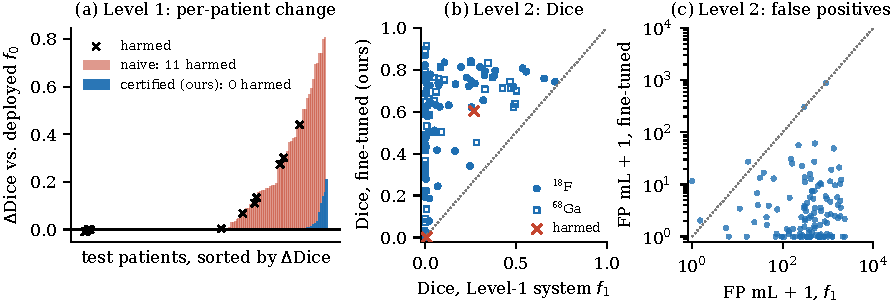
\includegraphics[width=\linewidth]{fig/fig_patients.pdf}
  \caption{\textbf{Every locked test patient.}
  (a) Level 1: per-patient Dice change relative to the deployed agent, sorted; $\times$ marks harmed patients. Naive selection harms 11 patients, all by lost lesions, 7 of them while \emph{raising} their Dice; certified \ours harms none.
  (b) Level 2: per-patient Dice of the Level-1 system and of the certified fine-tuned segmenter ($^{18}$F filled, $^{68}$Ga open; red $\times$: the three harmed patients).
  (c) Level 2: per-patient false-positive volume (log scale).}
  \label{fig:patients}
\end{figure*}

\subsection{Does the certificate keep its promise?}
\label{sec:validity}
A single test set is one draw.
To measure how often each selection rule breaks its promise, we resample the 251 patients of $\B\cup\C$ into 1,000 random halves, select on one half and measure the realised harm rate on the other, with detectors fixed.
\Cref{fig:validity} shows the violation frequency $\Pr[\hat R>\delta]$ at $\delta=0.05$.
Certified selection violates in 0.2--0.5\% of splits on all three segmentation backbones, within $\alpha=5\%$; naive selection violates in 98.5--99.6\%.
At $\delta=0.10$ the rates are 0.3--0.7\% against 35--52\%.
The same holds in the source domain: on 630 FDG patients, naive selection breaks a 2\% promise in 76.6\% of splits and certified selection in 0.8\%.
Naive selection is not merely riskier; its stated risk is wrong.

\begin{figure}[t]
  \centering
  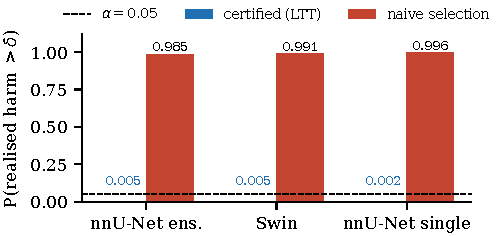
\includegraphics[width=\linewidth]{fig/fig_validity.pdf}
  \caption{\textbf{Validity.} Fraction of 1,000 random selection/evaluation splits of $\B\cup\C$ in which the realised harm rate exceeds the promised $\delta=0.05$, for three segmentation backbones.}
  \label{fig:validity}
\end{figure}

\subsection{The risk--benefit dial}
\label{sec:dial}
\Cref{fig:dial} sweeps the tolerance for the Level-1 agent updates, certifying on $\B$ and measuring on the locked $\C$.
At $\delta=0.03$ nothing is certifiable at $n=126$ (\cref{sec:ltt}) and the system rolls back; from $\delta=0.05$ to $0.20$ the summed benefit grows from $+0.79$ to $+4.63$ Dice-points, approaching naive selection ($+5.63$) while the realised harm rate stays below $\delta$ at every setting.
At Level 2 the dial is a step: rollback at $\delta=0.05$, the fine-tuned segmenter from $\delta=0.10$ on.
The dial does not tell a site which tolerance to choose; it tells it, before deployment, what each tolerance buys.

\para{The price of a guarantee.}
With 4 harmed of 126, the Level-2 switch is certifiable for any $\delta\ge0.080$ (\cref{fig:power}b).
The same 4 harms would certify $\delta=0.05$ among 202 certification patients; a 1\% guarantee needs at least 368 patients even if none is harmed (\cref{fig:power}a, \cref{tab:supp_n}).
A site can compute this cost before it labels a single case.

\begin{figure}[t]
  \centering
  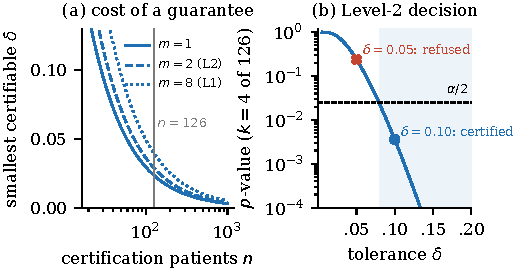
\includegraphics[width=\linewidth]{fig/fig_power.pdf}
  \caption{\textbf{The price of a guarantee.} (a) Smallest certifiable tolerance with zero observed harms, $1-(\alpha/m)^{1/n}$, against the number of certification patients, for $m$ chains ($\alpha=0.05$). (b) Level-2 $p$-value on $\B$ (4 of 126 patients harmed) against $\delta$; the switch is certified where $p\le\alpha/2$ (shaded).}
  \label{fig:power}
\end{figure}

\begin{figure}[t]
  \centering
  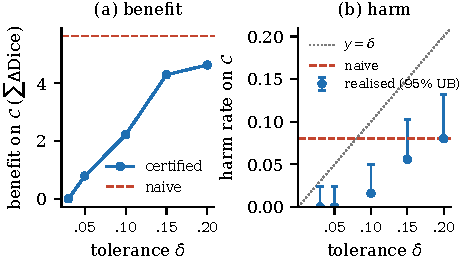
\includegraphics[width=\linewidth]{fig/fig_dial.pdf}
  \caption{\textbf{Risk--benefit dial} (Level 1, locked $\C$). (a) Summed Dice benefit of the certified update as the tolerance $\delta$ grows; naive selection dashed. (b) Realised harm rate with 95\% upper bound, against $y=\delta$. Computed from per-action outcomes rather than an end-to-end agent run, so the naive point harms 10 patients, not the 11 of \cref{tab:main}.}
  \label{fig:dial}
\end{figure}

\begin{table}[t]
\centering
\caption{\textbf{Generality across segmenters} (Level 1, locked $\C$, $\delta=0.05$). Benefit is relative to the deployed agent on the same segmenter. $\dagger$: safety not confirmed after the pre-registered Holm correction over the two secondary backbones ($p=0.048>0.025$).}
\label{tab:backbones}
\setlength{\tabcolsep}{3.4pt}
\small
\begin{tabular}{@{}lccc@{}}
\toprule
segmenter & harmed (UB) & $\Delta$Dice {\scriptsize[95\% CI]} & $\Delta$FP mL \\
\midrule
nnU-Net, 5-fold & 0 (2.4\%) & \makecell{$+0.0068$\\[-2pt]{\scriptsize[$+0.0022$, $+0.0126$]}} & $-127$ \\
Swin & 2 (5.0\%)$^\dagger$ & \makecell{$+0.0055$\\[-2pt]{\scriptsize[$+0.0011$, $+0.0123$]}} & $-163$ \\
nnU-Net, single & 2 (5.0\%)$^\dagger$ & \makecell{$+0.0012$\\[-2pt]{\scriptsize[$+0.0003$, $+0.0026$]}} & $-68$ \\
\bottomrule
\end{tabular}
\end{table}

\subsection{Generality across segmenters}
\label{sec:generality}
We repeat Level-1 certification on two further PSMA segmenters, a Swin-transformer backbone~\cite{liu2021swin} and a single nnU-Net model (\cref{tab:backbones}).
The Dice benefit and the FP reduction replicate on both ($p<0.001$ each).
Each harms 2 of 125 test patients (1.6\%, below $\delta$), but with the pre-registered Holm correction the safety endpoint is not confirmed on either, and each loses 2 lesion detections.
Validity (\cref{fig:validity}) holds on all three.

\section{Discussion and Limitations}
\label{sec:discussion}

\para{What the certificate does, and does not, do.}
The certificate does not make an update better; it makes its risk \emph{known and bounded} before deployment.
In our data that distinction decided every outcome.
Naive selection always looked best on average and always broke its promise; certified selection was sometimes less ambitious and kept it.
Where benefit was large (Level 2), the certificate did not stand in the way of it; it priced it, in units a clinician can reason about: ``5\% is not supported by 126 patients; 10\% is.''

\para{Where the gain comes from.}
Self-improvement of the refinement agent was safe but worth $+0.009$ Dice; self-improvement of the segmenter on the same 126 patients was worth $+0.44$.
An agent that edits a segmentation can remove what is wrong but cannot supply what is missing.
We consider this a useful negative result for the growing literature on self-refining systems: under a large domain shift, refinement is no substitute for adapting the model, and a certificate is what makes adapting the model deployable.

\para{Limitations.}
\textbf{(1) Primary endpoint at Level 2.} The pre-registered $\delta=0.05$ switch was not certified; the Level-2 gain is certified at $\delta=0.10$, a pre-registered dial setting, and we report it as such.
\textbf{(2) Test reuse.} $\C$ was read for Level 1 before Level 2 was planned. No Level-2 decision used $\C$, but a fresh test set would be stronger.
\textbf{(3) Sample size.} With 126 certification patients the smallest certifiable tolerance is about 4\%; clinical tolerances near 1\% need several hundred patients per site.
\textbf{(4) Harm definition.} Harm is relative to the deployed system and counts a lesion as detected on any overlap, so a system with large false-positive regions ``detects'' lesions by accident (\cref{fig:qual}d). We kept the pre-registered definition; a minimum-overlap criterion would be clinically more faithful.
\textbf{(5) Generality.} Safety on the two secondary backbones is consistent with, but not confirmed at, the corrected level, and both lose two lesion detections.
\textbf{(6) Scope.} One shift (FDG$\to$PSMA), one disease, retrospective data; exchangeability between certification and future patients is assumed and would fail under further drift, which calls for re-certification.
\textbf{(7) Absolute accuracy.} A fine-tuned Dice of 0.55 on 126 patients is below models trained on the full PSMA cohort; our contribution is the update protocol, not a new state of the art.

\para{Conclusion.}
Self-improvement need not be a leap of faith.
Stating, in advance, how many patients an update may harm, testing that statement on held-out patients, and rolling back when the evidence is insufficient turned an FDG segmentation system into a PSMA one with a five-fold Dice gain and a bounded, verified risk---and exposed exactly why the obvious alternatives are unsafe.
We will release code, pre-registration documents and lock files.

\section*{LLM Usage Statement}
\label{sec:llm}
\CHECK{authors: confirm this text against the CVPR 2027 LLM policy and your own use; edit before submission}

A large language model (LLM) coding assistant was used throughout this project, under the authors' direction and review.
\textbf{Code.} It wrote and edited analysis, training-orchestration, evaluation and figure scripts; every script was run by the authors' pipeline on the authors' machine, and every number in the paper is produced by those scripts from locked result files, not typed by the model.
\textbf{Protocol.} It drafted pre-registration plans and lock files, which the authors reviewed and committed before the corresponding numbers were computed; the study design, the harm definition, the tolerances and all go/no-go decisions are the authors'.
\textbf{Writing.} It drafted and edited text of this paper and its supplement, which the authors revised and verified against the result files.
\textbf{Data.} Only de-identified public datasets were processed; no patient data were collected.
The LLM is not an author; the authors take full responsibility for the content, including any errors.
References were checked by the authors; the LLM was instructed not to add citations it could not verify.


{
    \small
    \bibliographystyle{ieeenat_fullname}
    \bibliography{main}
}

\ifwithsuppl
\clearpage
\setcounter{page}{1}
\setcounter{section}{0}
\renewcommand{\thesection}{S\arabic{section}}
\renewcommand{\thetable}{S\arabic{table}}
\renewcommand{\thefigure}{S\arabic{figure}}
\setcounter{table}{0}
\setcounter{figure}{0}
\maketitlesupplementary

\noindent This supplement contains the guarantee's proof and power analysis (\cref{sec:supp_proof}), the refinement agent (\cref{sec:supp_agent}), the full Level-1 (\cref{sec:supp_level1}) and Level-2 (\cref{sec:supp_level2}) results, zero-shot transfer and subgroups (\cref{sec:supp_zeroshot}), source-domain development and its negative results (\cref{sec:supp_fdg}), the pre-registration ledger and every deviation (\cref{sec:supp_deviations}), and reproducibility details (\cref{sec:supp_repro}).

%----------------------------------------------------------------------------
\section{Guarantee and power}
\label{sec:supp_proof}

\para{Proof of \cref{thm:ltt}.}
Fix $\lambda$ with $R(\lambda)>\delta$. The harms $H_i(\lambda)$, $i\in\B$, are i.i.d.\ Bernoulli($R(\lambda)$) because $\Lam$ is built without $\B$ and patients are exchangeable; hence $k_\lambda$ is stochastically larger than $\mathrm{Bin}(n,\delta)$ and $\Pr[p_\lambda\le u]\le u$ for all $u\in[0,1]$.
Within a chain $\lambda_{1}\prec\lambda_{2}\prec\dots$ (fixed before $\B$ is seen), fixed-sequence testing at level $\alpha/m$ rejects $\lambda_j$ only if $p_{\lambda_1},\dots,p_{\lambda_j}\le\alpha/m$; the first true null in the sequence is rejected with probability at most $\alpha/m$, and no later hypothesis is tested unless it is, so the chain's family-wise error is at most $\alpha/m$~\cite{bretz2010multiple}.
A union bound over $m$ chains gives $\Pr[\exists\lambda\in\hat\Lam: R(\lambda)>\delta]\le\alpha$.
The deployed $\hat\lambda$ is an element of $\hat\Lam$ or the rollback ($R=0$); choosing among $\hat\Lam$ by any data-dependent benefit cannot leave the event above, so $\Pr[R(\hat\lambda)>\delta]\le\alpha$. \hfill$\square$

\para{What the assumptions mean here.}
(i) Level-1 candidates are fitted on $\A$ (detectors and isotonic calibrators by 5-fold cross-fitting within $\A$; the out-of-distribution fence from $\A$'s component counts) and on source-domain data; Level-2 candidates are trained on $\A$ only. $\B$ is used for nothing but the test and the benefit-based choice among certified candidates.
(ii) Exchangeability holds by construction for $\B$ and $\C$ (one random split, stratified by radionuclide $\times$ tumour status); for future patients it is an assumption.
(iii) At Level 1, $H_i$ on $\B$ is computed from the \emph{measured} outcome of each added action on each component (a lesion lost or a tumour-positive Dice drop $>0.01$), and a patient counts as harmed if any added component is harmful. The deployed agent applies actions sequentially, so the test-set harm in \cref{tab:main} is measured on the actual agent output, not on this component-wise proxy; both agree on $\C$ (0 harmed).

\para{Power.} With zero observed harms, $H_\lambda$ is rejected iff $(1-\delta)^n\le\alpha/m$.
\Cref{tab:supp_power} lists the smallest certifiable tolerance.

\begin{table}[h]
\centering
\caption{Smallest certifiable tolerance $\delta_{\min}=1-(\alpha/m)^{1/n}$ at $\alpha=0.05$.}
\label{tab:supp_power}
\small
\begin{tabular}{@{}rccc@{}}
\toprule
$n$ & $m=1$ & $m=2$ (Level 2) & $m=8$ (Level 1) \\
\midrule
126 & 0.024 & 0.029 & 0.040 \\
250 & 0.012 & 0.015 & 0.020 \\
500 & 0.006 & 0.007 & 0.010 \\
1000 & 0.003 & 0.004 & 0.005 \\
\bottomrule
\end{tabular}
\end{table}

%----------------------------------------------------------------------------
\section{The refinement agent}
\label{sec:supp_agent}

\para{Candidates and features.}
The segmenter's probability map $P$ is thresholded at 0.5; each connected component is a candidate for repair, and components of $P>0.1$ not touching the mask are candidates for recovery.
Each component is described by 26 observable features (volume, SUV statistics, shape, position, predicted-probability and uncertainty statistics from the ensemble, distance to organs) and, for the context detector, 21 more: local contrast (shell SUV mean, tumour-to-background ratios), edge sharpness, uptake texture, CT texture and air/bone fractions, the fraction of the shell in physiological-uptake organs and liver, model-probability profile in the shell, and left--right mirror SUV ratio. No feature uses ground truth.

\para{Failure classes and detectors.}
Eight classes are predicted per component: spurious (physiological / liver--spleen / other), merging, under-segmentation, over-segmentation, boundary error and fragmentation; a separate head predicts missed lesions for recovery candidates.
Labels come from matching components to ground truth.
Each class head is a gradient-boosted classifier (scikit-learn \texttt{HistGradientBoostingClassifier}, depth 3, learning rate 0.08, 200 iterations).
``Old'' uses the 26 features; ``new'' adds the 21 context features; ``ens'' averages the calibrated old and new probabilities.
Calibration is isotonic regression fitted on cross-fitted predictions only.

\para{Actions and the hand-built policy.}
For the predicted (argmax) class, the policy applies the first applicable action of a fixed list (\cref{tab:supp_policy}). Actions: \emph{remove} (delete the component), \emph{fill} (fill holes), \emph{merge} (close a gap of 2 voxels to a neighbour), \emph{boundary} (re-threshold $P$ at 0.5 in a 2-voxel shell), \emph{SUV41} (re-threshold at 41\% of the component's SUV$_{\max}$), \emph{PERCIST} (re-threshold at the liver-referenced PERCIST level), \emph{grow} (dilate into $P>0.3$), \emph{shrink} (keep $P>0.7$), \emph{recover} (add a recovery candidate).
The agent acts once per component, up to $T=10$ iterations per scan, and only when the detector's max-class probability passes the gate (0.90 for the hand-built agent).

\begin{table}[h]
\centering
\caption{Hand-built policy: ordered actions per predicted class.}
\label{tab:supp_policy}
\footnotesize
\begin{tabular}{@{}ll@{}}
\toprule
class & actions (first applicable is used) \\
\midrule
spurious, physiological & PERCIST, SUV41, remove, shrink \\
spurious, liver/spleen & remove, PERCIST, SUV41, shrink \\
spurious, other & remove, PERCIST, shrink \\
under-segmentation & grow, merge, SUV41, boundary \\
over-segmentation & fill \\
fragmentation & grow, merge, boundary \\
merging & fill \\
boundary & grow, boundary, fill \\
missed & recover \\
\bottomrule
\end{tabular}
\end{table}

\para{Anchored updates and guards.}
A Level-1 update keeps every hand-built action and may add actions on components the hand-built agent leaves alone (one-sided trust region). An addition requires the chosen detector's calibrated max-class probability $\ge t$, the component's scan to be inside the out-of-distribution fence (component count $\le Q_3+3\,\mathrm{IQR}$ on $\A$; 52 for the primary segmenter), and the chosen guard: \emph{agree} (old and new argmax classes agree and the old calibrated max-class probability is $\ge0.5$), \emph{solo} (never act on a scan's only component), both, or none.
Benefit for selection among certified candidates is the summed measured Dice change of the added actions; a candidate also needs $\ge20$ additions and a positive patient-clustered lower confidence bound on mean benefit.

%----------------------------------------------------------------------------
\section{Level 1: full results}
\label{sec:supp_level1}

\para{Certification on $\B$.} \Cref{tab:supp_chains} gives the number of harmed $\B$ patients for every candidate. At $\alpha/8$ only $k=0$ rejects; 22 candidates are certified. The selected update is the calibrated new detector at gate 0.97 with both guards (64 additions, summed benefit $+0.28$ on $\B$). Naive selection picks the most aggressive candidate (new detector, gate 0.85, no guard): 13 harmed patients and 22 lost lesions on $\B$.

\begin{table*}[t]
\centering
\caption{Harmed patients on $\B$ ($n=126$) per Level-1 candidate (primary segmenter). $\ast$: certified at $\delta=0.05$, $\alpha/8$.}
\label{tab:supp_chains}
\footnotesize
\setlength{\tabcolsep}{4pt}
\begin{tabular}{@{}llccccccccccc@{}}
\toprule
detector & guard & 0.99 & 0.98 & 0.97 & 0.96 & 0.95 & 0.94 & 0.93 & 0.92 & 0.91 & 0.90 & 0.85 \\
\midrule
new, cal. & none & 1 & 2 & 2 & 2 & 2 & 5 & 5 & 7 & 7 & 7 & 13 \\
new, cal. & solo & 1 & 2 & 2 & 2 & 2 & 5 & 5 & 7 & 7 & 7 & 13 \\
new, cal. & agree & 0$^\ast$ & 0$^\ast$ & 0$^\ast$ & 0$^\ast$ & 0$^\ast$ & 3 & 3 & 5 & 5 & 5 & 5 \\
new, cal. & agree+solo & 0$^\ast$ & 0$^\ast$ & 0$^\ast$ & 0$^\ast$ & 0$^\ast$ & 3 & 3 & 5 & 5 & 5 & 5 \\
ens & any of 4 & 0$^\ast$ & 0$^\ast$ & 0$^\ast$ & 1 & 1 & 1 & 1 & 3 & 3 & 3 & 3 \\
\bottomrule
\end{tabular}
\end{table*}

\para{Dial on $\C$ for all backbones.} \Cref{tab:supp_dial} lists, per tolerance, the update certified on $\B$ and its outcome on $\C$. On the primary segmenter the realised rate never exceeds $\delta$. On the secondary segmenters it does at some settings (Swin, $\delta=0.15$: 0.096; nnU-Net single, $\delta=0.15$: 0.112), within the binomial noise of 125 patients but not uniformly below $\delta$.

\begin{table}[h]
\centering
\caption{Level-1 dial: certified on $\B$, measured on $\C$ ($n=125$). Benefit: summed Dice change of added actions; $k$: harmed patients.}
\label{tab:supp_dial}
\footnotesize
\setlength{\tabcolsep}{3.5pt}
\begin{tabular}{@{}lcccccc@{}}
\toprule
& \multicolumn{2}{c}{nnU-Net ens.} & \multicolumn{2}{c}{Swin} & \multicolumn{2}{c}{nnU-Net single} \\
\cmidrule(lr){2-3}\cmidrule(lr){4-5}\cmidrule(lr){6-7}
$\delta$ & benefit & $k$ & benefit & $k$ & benefit & $k$ \\
\midrule
0.03 & rollback & 0 & rollback & 0 & rollback & 0 \\
0.05 & $+0.79$ & 0 & $+0.32$ & 2 & $+0.14$ & 2 \\
0.10 & $+2.22$ & 2 & $+2.01$ & 4 & $+0.62$ & 4 \\
0.15 & $+4.29$ & 7 & $+4.48$ & 12 & $+3.39$ & 14 \\
0.20 & $+4.63$ & 10 & $+4.53$ & 14 & $+3.57$ & 15 \\
naive & $+5.63$ & 10 & $+4.53$ & 14 & $+3.57$ & 15 \\
\bottomrule
\end{tabular}
\end{table}

\para{Validity at both tolerances.} \Cref{tab:supp_validity} adds mean realised risk and benefit to \cref{fig:validity}.

\begin{table}[h]
\centering
\caption{Validity over 1,000 random halves of $\B\cup\C$: violation rate $\Pr[\hat R>\delta]$, mean realised risk and mean summed benefit, certified (LTT) / naive.}
\label{tab:supp_validity}
\footnotesize
\setlength{\tabcolsep}{3pt}
\begin{tabular}{@{}llccc@{}}
\toprule
backbone & $\delta$ & violation & mean risk & mean benefit \\
\midrule
nnU-Net ens. & 0.05 & 0.005 / 0.985 & 0.010 / 0.092 & $+0.83$ / $+5.95$ \\
 & 0.10 & 0.004 / 0.350 & 0.031 / 0.092 & $+3.50$ / $+5.95$ \\
Swin & 0.05 & 0.005 / 0.991 & 0.011 / 0.095 & $+0.61$ / $+5.61$ \\
 & 0.10 & 0.007 / 0.415 & 0.037 / 0.095 & $+2.63$ / $+5.61$ \\
nnU-Net single & 0.05 & 0.002 / 0.996 & 0.004 / 0.100 & $+0.38$ / $+4.19$ \\
 & 0.10 & 0.003 / 0.516 & 0.041 / 0.100 & $+1.40$ / $+4.19$ \\
\bottomrule
\end{tabular}
\end{table}

\para{Additional Level-1 outcomes on $\C$ (primary).} Against the deployed agent: HD95 198.0$\to$194.0\,mm; 46 of 125 scans changed; tumour-free scans cleared of all FP 0 vs.\ 0 of 6 (the pre-registered clearance endpoint had no power with 6 tumour-free patients). FP-volume intervals for all arms: certified $-126.7$ [$-185.8$, $-74.4$], uncalibrated $-214.0$ [$-284.4$, $-150.3$], naive $-523.1$ [$-631.6$, $-420.3$], pseudo-label $+20.8$ [$+13.0$, $+28.7$] mL per scan (case bootstrap, 5,000 resamples).

%----------------------------------------------------------------------------
\section{Level 2: full results}
\label{sec:supp_level2}

\para{Recipe (fixed in the plan, not tuned).} nnU-Net v2, 3D full resolution, plans and network of the source model (patch $192\times96\times128$, spacing $3\times2.04\times2.04$\,mm, batch 2, plain convolutional U-Net with 6 stages). Five folds over $\A$ (101/25 patients); each fold starts from a different one of the five source models, with all weights including the segmentation head; SGD with nnU-Net's poly schedule from learning rate $3\times10^{-3}$, 100 epochs of 250 iterations, final checkpoint. Out-of-fold validation Dice on $\A$ per fold: 0.489, 0.436, 0.582, 0.434, 0.422 (not used for any decision). $\B$ and $\C$ are predicted by the 5-fold ensemble with 8-fold flip averaging, exactly as the source model.

\para{Certification on $\B$.} \Cref{tab:supp_l2b}. The four harmed $\B$ patients: hits 12$\to$6 (Dice 0.18$\to$0.08); hits 3$\to$2 (Dice 0.01$\to$0.59); hits 16$\to$9 (Dice 0.69$\to$0.46); Dice 0.50$\to$0.06 with hits unchanged.

\begin{table}[h]
\centering
\caption{Level 2 on $\B$ ($n=126$), reference: the Level-1 system. Each candidate tested at $\alpha/2$.}
\label{tab:supp_l2b}
\footnotesize
\setlength{\tabcolsep}{3.5pt}
\begin{tabular}{@{}lcccccc@{}}
\toprule
 & Dice & harmed & $p_{\delta=.05}$ & $p_{\delta=.10}$ & $p_{\delta=.15}$ & deployed at \\
\midrule
Level-1 system & 0.122 & -- & -- & -- & -- & $\delta=0.05$ \\
FT & 0.571 & 4 & 0.240 & 0.004 & $<10^{-4}$ & $\delta\ge0.10$ \\
FT+agent & 0.570 & 4 & 0.240 & 0.004 & $<10^{-4}$ & -- \\
\bottomrule
\end{tabular}
\end{table}

\para{Agent on top of the fine-tuned segmenter.} Re-running Level-1 certification on the fine-tuned maps (detectors adapted on out-of-fold $\A$ predictions) certified no addition; the system rolls back to the hand-built agent on top of FT, whose test table is byte-identical to FT+agent in \cref{tab:main}. FT+agent clears 3 of 6 tumour-free test patients of all false positives, FT alone 1.

\para{Harmed test patients} (FT vs.\ Level-1 system): (i) 1 lesion, hit 1$\to$0, Dice 0.011$\to$0.000, FP 10$\to$2\,mL; (ii) 2 lesions, hits 2$\to$0, Dice 0.011$\to$0.000, FP 94$\to$0\,mL; (iii) 120 lesions, hits 106$\to$102, Dice 0.271$\to$0.603, FP 314$\to$3\,mL. In (i) and (ii) the Level-1 system overlapped the lesions only as part of large false-positive regions.

%----------------------------------------------------------------------------
\section{Zero-shot transfer and subgroups}
\label{sec:supp_zeroshot}

Before any adaptation, the frozen source agent and its source-certified update (certified at $\delta=0.01$ on 630 FDG patients) were run on all 377 PSMA patients under a pre-registered lock. Primary endpoints: harmed 0/377 ($p=0.023$ against $R>0.01$; UB 0.79\%), Dice and lesion non-inferiority met. Benefit was nil: the update changed 7 scans; both arms improved Dice over the bare segmenter by $+0.0013$ [$+0.0006$, $+0.0022$]. The certified update abstained (out-of-fence) on 67 scans. \Cref{tab:supp_subgroups} shows that harm was zero in every subgroup and that the largest disparity is in the base segmenter, not the agent.

\begin{table}[h]
\centering
\caption{Zero-shot transfer by subgroup (all 377 PSMA patients). Harmed patients: 0 in every subgroup.}
\label{tab:supp_subgroups}
\footnotesize
\begin{tabular}{@{}lccc@{}}
\toprule
subgroup & $n$ & segmenter Dice & agent $-$ segmenter \\
\midrule
$^{18}$F & 213 & 0.111 & $+0.0002$ \\
$^{68}$Ga & 164 & 0.109 & $+0.0027$ \\
vendor 1 & 157 & 0.056 & $+0.0012$ \\
vendor 2 & 220 & 0.147 & $+0.0014$ \\
age, lowest tertile & 133 & 0.100 & $+0.0020$ \\
age, middle & 135 & 0.102 & $+0.0006$ \\
age, highest & 109 & 0.131 & $+0.0012$ \\
\bottomrule
\end{tabular}
\end{table}

%----------------------------------------------------------------------------
\section{Source-domain development and negative results}
\label{sec:supp_fdg}

The agent was developed over many pre-registered phases on FDG data. We report the ledger because the negative results shaped the design and because a reader should know how many things were tried.

\para{Confirmatory source result.} The iterative, confidence-gated agent improved test Dice over the 5-fold segmenter by $+0.0067$ [$+0.0012$, $+0.0164$] (200 test patients, single pre-registered test pass), cleared 6 of 90 tumour-free patients of false positives and degraded none.

\para{Negative and mixed results} (all pre-registered):
(1) A learned quality critic (predicted Dice) adjudicated single actions at 37.1\% precision, below its 60\% threshold; a loop gated by it accepted no action.
(2) Learned strategy selection did not beat the fixed hand-built strategy at matched budget; experience-based self-improvement curves were flat.
(3) Learned action gates, class-specific gates, an experience-trained harm model, KL-anchored policy improvement, a context detector, calibration with guards, and out-of-distribution abstention each failed to beat the hand-built policy on its pre-registered criteria; the first update to pass every out-of-fold endpoint (descriptively) was the LTT-certified anchored union used here.
(4) Gains concentrate, narrowly, in the hardest cases.

\para{LTT in the source domain.} Certifying on 630 out-of-fold patients ($\delta=0.01$, $\alpha=0.05$) certified 36 of 88 candidates; the deployed update added 48 actions with 0 harmed patients. Source dial (out-of-fold, descriptive): $\delta=0.01$: $+4.47$ summed benefit, 0 harmed; $0.02$: $+13.63$, 4; $0.03$: $+16.77$, 6; $0.05$: $+25.38$, 18. On the locked source test set (200 patients) the update changed 5 scans and harmed none (UB 1.5\%); its gain was too small to be significant. Validity on 1,000 halves: violation 0.008 vs.\ 0.766 (naive) at $\delta=0.02$; 0.010 vs.\ 0.402 at $0.03$; 0.007 vs.\ 0.007 at $0.05$.

%----------------------------------------------------------------------------
\section{Pre-registration, locks and deviations}
\label{sec:supp_deviations}

\para{Ledger.} Each phase had a committed plan (candidates, $\delta$, $\alpha$, endpoints, failure criteria) before its numbers were computed, and a lock (SHA-256 of every test input and the exact commands) before its test set was read. The PSMA phases are: zero-shot transfer (one lock), Level 1 (one lock for the primary segmenter, one for the two secondary segmenters), Level 2 (one lock). Plans and locks will be released with timestamps.

\para{Deviations and corrections.}
\begin{enumerate}[nosep,leftmargin=*]
\item \textbf{Level-2 primary not met.} The switch was not certified at $\delta=0.05$ and the pre-registered rule rolled back; the reported gain is the pre-registered $\delta=0.10$ dial setting.
\item \textbf{Test reuse.} $\C$ was read for the Level-1 arms before the Level-2 plan was written; no Level-2 decision used $\C$.
\item \textbf{Per-segmenter locks.} The Level-1 plan described one lock; the secondary segmenters' predictions were not ready, so each segmenter was locked separately before its own test run.
\item \textbf{Zero-shot run restarts.} Two runs aborted on a patient-identifier lookup before writing any output; input hashes were re-verified before the run that counts.
\item \textbf{File collision.} Two evaluation scripts wrote the same file name; the overwritten, deterministic evaluation was re-run and gave identical numbers.
\item \textbf{FP-volume intervals} were computed after the lock with a case bootstrap, because the evaluation script printed only means.
\item \textbf{Subgroup artefact.} One evaluation flagged a ``mid-difficulty'' subgroup defined by source-domain tertiles; on PSMA it contains one patient whose Dice change is exactly zero.
\item \textbf{Erratum.} A Level-1 lock note stated that 40 of 88 candidates were certified; the certification output (and this paper) has 22. The deployed configuration, computed by code, is unaffected.
\item \textbf{$p$-values.} Bootstrap $p$ for Dice differences is two-sided (conservative for the one-sided endpoints) with a floor of $1/2000$.
\end{enumerate}

%----------------------------------------------------------------------------
\section{Reproducibility}
\label{sec:supp_repro}

\para{Data.} AutoPET FDG PET/CT and PSMA-PET-CT-Lesions are public on TCIA under their data-usage policies; PSMA-PET-CT-Lesions is CC BY 4.0. Two PSMA studies failed conversion and were excluded before any analysis. No new human-subject data were collected.

\para{Compute.} One NVIDIA RTX 5000 Ada (32\,GB). Level-2 fine-tuning: about 1.8\,h per fold, 9\,h in total; ensemble inference on 251 patients: about 3\,h. Detectors, certification and the agent run on CPU (about 7--10\,s per scan for the agent).

\para{Release.} Code, pre-registration plans, lock files and per-patient result tables will be released upon publication.

\fi

\end{document}
